\subsection{if\_file\_not\_founded()}

Блок-схема на рисунке \ref{fig:if_file_not_founded}.

\begin{figure}[p]
    \center{
        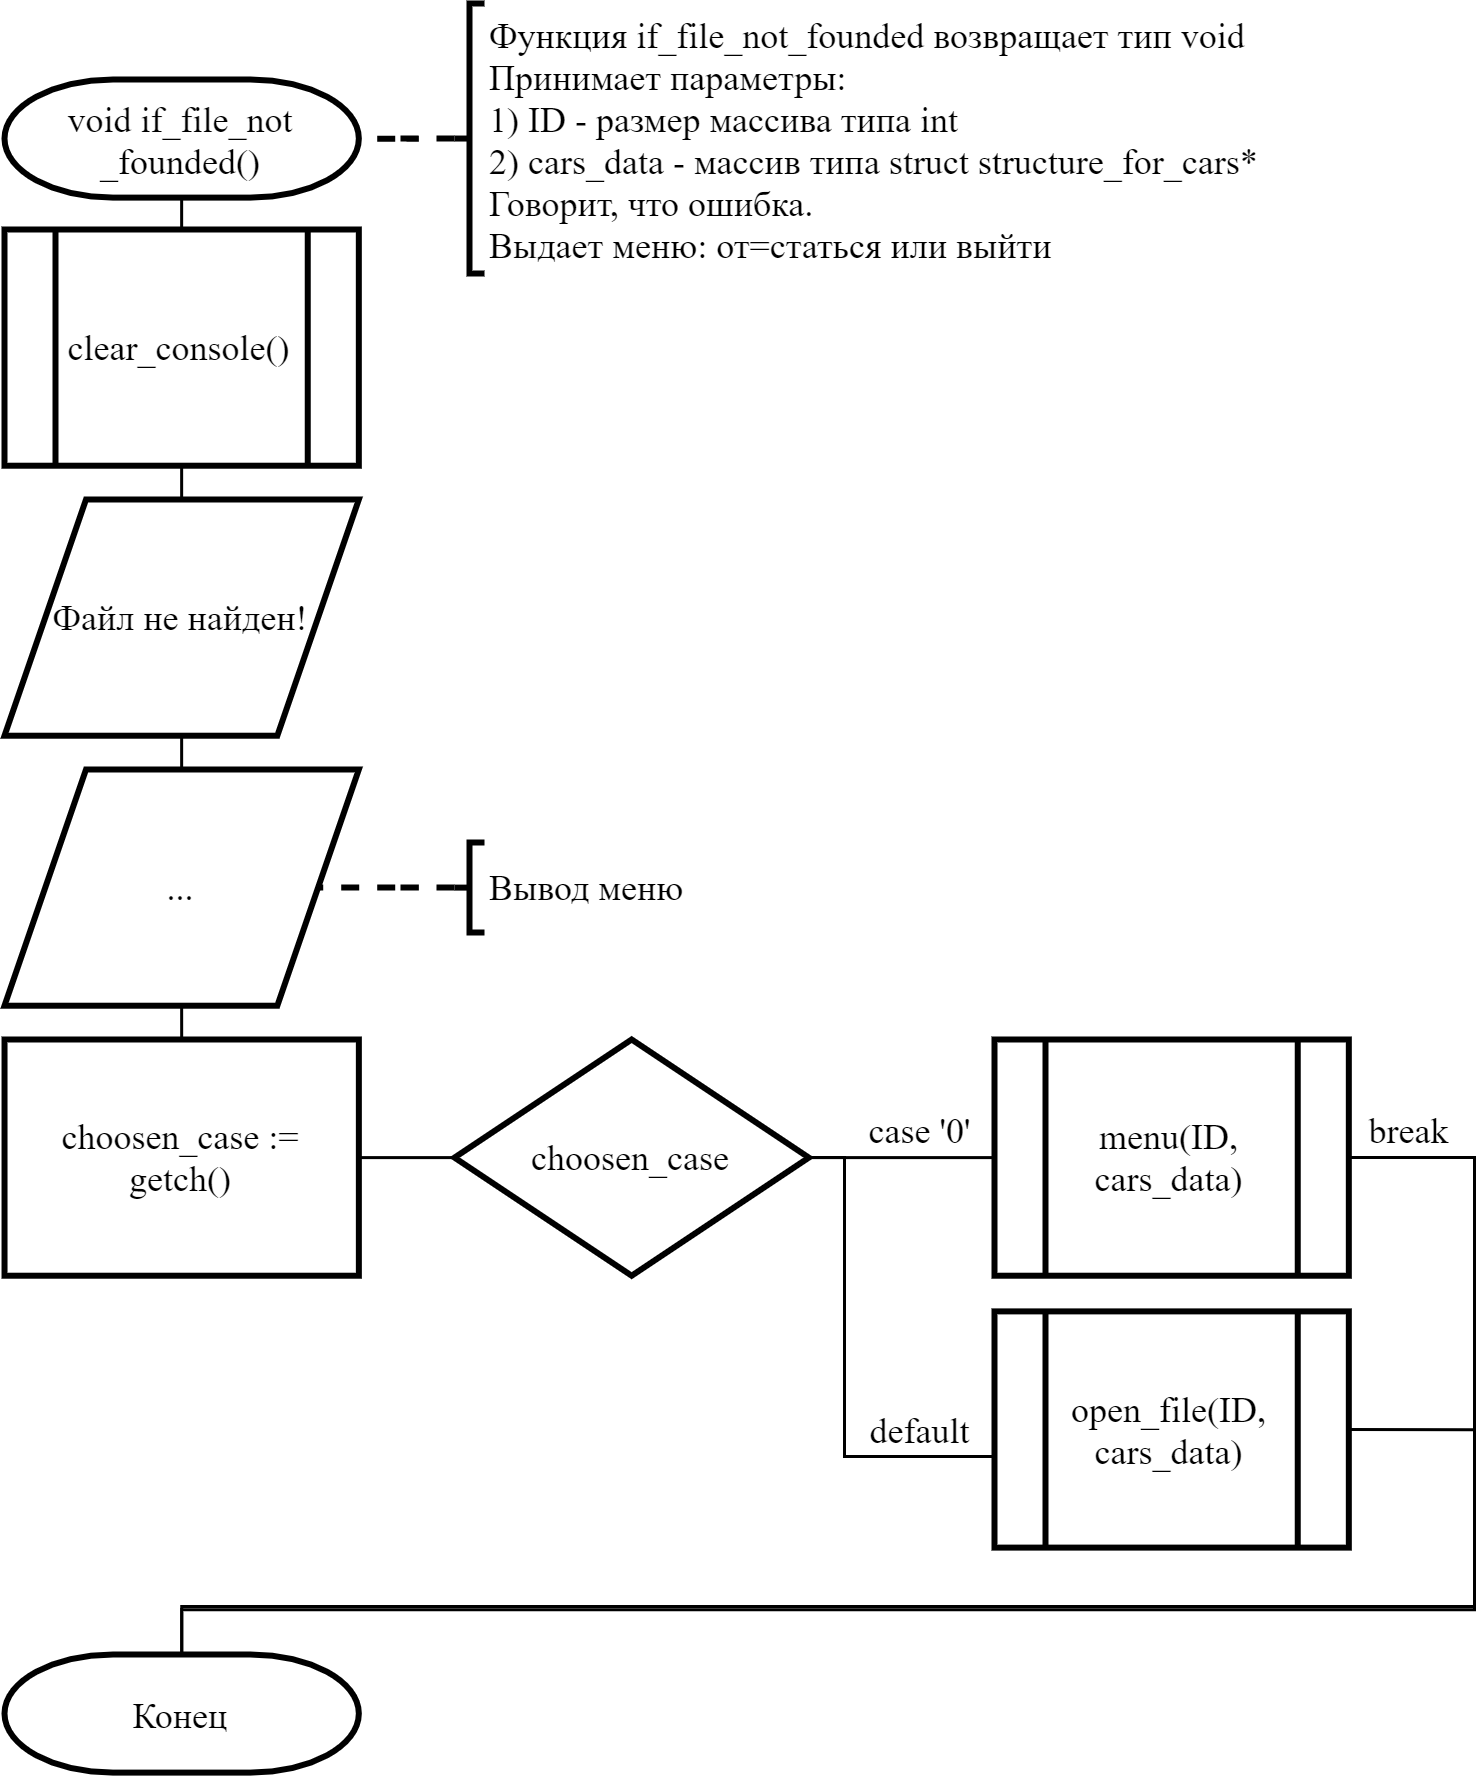
\includegraphics[]{../13/src/lab/menu/open_file/if_file_not_founded/if_file_not_founded.png}
    }
    \caption{if\_file\_not\_founded()}
    \label{fig:if_file_not_founded}
\end{figure}

\lstinputlisting[
    language=C,
    name=if\_file\_not\_founded.h
]{../13/src/lab/menu/open_file/if_file_not_founded/if_file_not_founded.h}

\lstinputlisting[
    language=C,
    name=if\_file\_not\_founded.c
]{../13/src/lab/menu/open_file/if_file_not_founded/if_file_not_founded.c}

\newpage